% Сгенерировано из lecture-04.md скриптом lecture-notes/scripts/finalize.py.
% Правки вносите в .md и запускайте finalize.py заново.
% Preamble for the final .tex of a ТЕНЗОРЫ lecture. scripts/finalize.py fills in the three
% placeholders; the body is generated from docs/lecture-NN/lecture-NN.md.
% Overleaf-compatible: compiles with Overleaf's default pdfLaTeX on TeX Live 2026, no project
% settings to change. Fonts are Computer Modern + cm-super (T2A), the same as the
% "Лекция 1. Индексы" example.
\documentclass[11pt,a4paper]{article}
\usepackage{cmap}                 % searchable/copyable Cyrillic in the PDF
\usepackage[T2A]{fontenc}
\usepackage[utf8]{inputenc}
\usepackage[russian]{babel}
\usepackage{amsmath,amssymb,amsthm,mathtools}
\usepackage[a4paper,left=2.2cm,right=2.2cm,top=2.6cm,bottom=2.4cm,headsep=0.8cm]{geometry}
\usepackage{fancyhdr}
\usepackage{graphicx}
\usepackage{float}
\usepackage[font=small,justification=centering]{caption}
\usepackage{array}
\usepackage{cancel}
\usepackage{enumitem}
\usepackage[hidelinks]{hyperref}

\pagestyle{fancy}
\fancyhf{}
\fancyhead[L]{ТЕНЗОРЫ}
\fancyhead[R]{Лекция 4. Линейные формы}
\fancyfoot[C]{\thepage}
\renewcommand{\headrulewidth}{0.4pt}

\setlength{\parindent}{1.5em}
\setlist{nosep, leftmargin=2em}
\renewcommand{\arraystretch}{1.15}

% Shorthands KaTeX knows natively, so drafts may use them. (\C is taken by T2A, so it is
% left out; write \mathbb{C}.)
\providecommand{\R}{\mathbb{R}}
\providecommand{\N}{\mathbb{N}}
\providecommand{\Z}{\mathbb{Z}}
\providecommand{\Q}{\mathbb{Q}}

% Header block: "Необходимые знания" / "О чем лекция".
\newenvironment{lectureabout}{\begin{list}{}{\leftmargin=2.2em\rightmargin=2.2em}\small\item[]}{\end{list}\medskip}
% Banner for drafts written without a transcript.
\newenvironment{draftnote}{\begin{center}\begin{minipage}{0.9\textwidth}\small\hrule\smallskip}{\smallskip\hrule\end{minipage}\end{center}}

\begin{document}

\begin{center}
  {\Large\bfseries Лекция 4. Линейные формы}
\end{center}
\medskip

\begin{lectureabout}
\textbf{Необходимые знания:} линейное пространство, линейная независимость, базис и размерность, изоморфизм линейных пространств (лекция 2); замена базиса и матрица перехода (лекция 3); символ Кронекера и действия с суммами (лекция 1); уравнение плоскости из аналитической геометрии.

\smallskip
\textbf{О чем лекция:} функции на линейном пространстве; линейные формы, их график и линии уровня; сопряжённое пространство $V^*$ и его размерность; взаимный базис; преобразование взаимного базиса и компонент линейной формы при замене базиса; откуда берутся верхние и нижние индексы.
\end{lectureabout}

От разгонных лекций мы переходим к серьёзным. Линейные формы — это первое знакомство с тензорами: линейная форма уже является одним из видов тензора, причём самым необходимым для их изучения. Конечно, изучив одни линейные формы, сказать, что мы знаем тензоры, ещё нельзя.

Напомним, на что мы опираемся. Мы работаем только с конечномерными линейными пространствами: $\dim V = n \in \mathbb{N}$. В таком пространстве существует базис $\{\vec e_i\}$ — ничего сверхъестественного, просто набор из $n$ линейно независимых элементов, по которому раскладывается любой элемент пространства. Выбор базиса порождает изоморфизм $V$ с пространством столбцов действительных чисел высоты $n$. Более того, все линейные пространства одной размерности изоморфны, т. е. «одинаково устроены»: их элементы можно спарить биекцией, сохраняющей сложение и умножение на число (если $a \leftrightarrow A$, $b \leftrightarrow B$ и $a + b = c$, то $c \leftrightarrow A + B$). Единственное, чем линейные пространства различаются, — размерность. В следующей лекции появится понятие канонического изоморфизма, без которого тензоров быть не может, и там мы будем обживаться с изоморфизмами на конкретных примерах.

В прошлой лекции обсуждалась замена базиса: четыре формулы, прямой и обратный переход для базисных векторов и для компонент вектора, причём где у базисных векторов стоит прямая матрица, у компонент стоит обратная, и наоборот. Сегодня мы снова встретимся с этими формулами и наконец поймём, откуда берутся верхние и нижние индексы. До сих пор все индексы писались снизу, и это ничему не мешало. С новой записью, как и с правилом суммирования Эйнштейна, торопиться не стоит: переходить на неё имеет смысл, когда чётко понимаешь, зачем она нужна.

\section{Функции на линейном пространстве}

\subsection{Куда отображать}

Линейное пространство — это в первую очередь множество и лишь во вторую очередь введённая на нём структура. А на множестве, как показывает практика, рано или поздно хочется строить функции, т. е. отображения из него куда-то. Куда можно отображать пространство $V$?

Первый напрашивающийся кандидат — само $V$: других пространств у нас пока нет. Но если представлять себе линейное пространство как мешок с элементами и двумя операциями, то при нём незаметно всегда был ещё один маленький мешочек — действительные числа. Они вшиты в само определение линейного пространства (умножение на число), а устроены проще, чем $V$. Поэтому начнём с функций
\[
f\colon V \to \mathbb{R}.
\]

Отображения $V \to V$ тоже появятся: если отобрать среди них самые простые, получатся тензоры. Вообще, тензорное исчисление — это наука о самых простых функциях, какие только можно построить.

Заметим, что отображаем мы в то самое числовое поле, над которым построено пространство. Мы работаем с вещественными линейными пространствами. Для пространства над полем комплексных чисел естественно было бы рассматривать функции $V \to \mathbb{C}$. Почему важно отображать именно в «свой» мешочек, станет видно при построении тензоров.

\subsection{Пример: длина вектора}

Чтобы понять, какими бывают такие функции, возьмём простое, но нетривиальное пространство — геометрические векторы на плоскости, отложенные от общей точки $0$. Чтобы это было линейное пространство, плоскость должна быть взята целиком, а не кусок её. Значения функции будем откладывать по третьей, вертикальной оси.

Самая напрашивающаяся функция на геометрических векторах — длина: $f(\vec a) = |\vec a|$. Чем дальше от нуля конец вектора, тем больше значение, и во всех направлениях одинаково; графиком получается конус (рис. 1).

\begin{figure}[H]
\centering
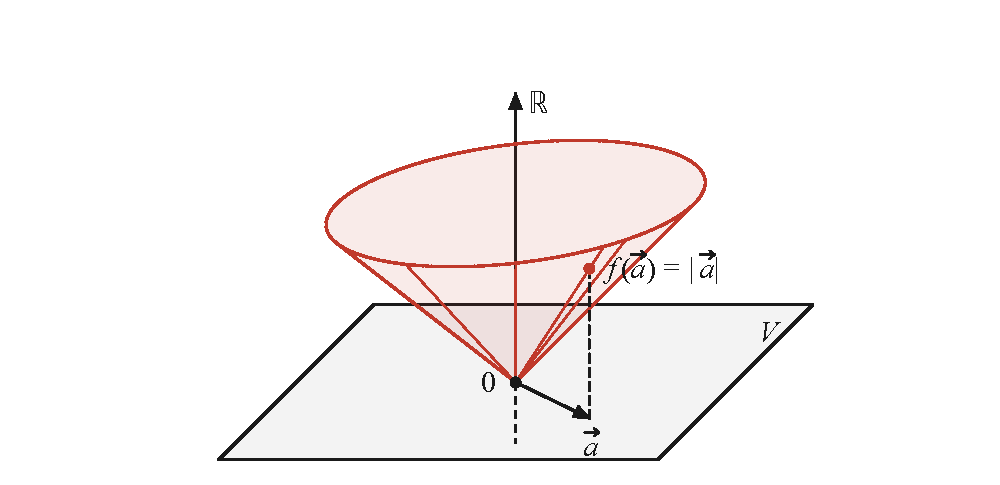
\includegraphics[width=0.84\textwidth]{figures/length-cone.pdf}
\caption*{Рис. 1. Функция «длина вектора» на плоскости геометрических векторов: над концом каждого вектора $\vec a$ на высоте $|\vec a|$ отмечено значение; все такие точки образуют конус.}
\end{figure}

Здесь мы воспользовались структурой, которой в линейном пространстве нет: оно не наделено ни длинами, ни углами, ни объёмами. У геометрических векторов эта более богатая структура есть, и запрещать себе ею пользоваться незачем. Но чтобы осознать общий факт сразу обо всех линейных пространствах, от неё полезно абстрагироваться: спросите прохожего, какова длина многочлена $x^2 + 1$, и он решит, что над ним издеваются (ввести скалярное произведение и назвать длиной корень из него можно, но это уже дополнительная структура).

Пример с конусом нужен для другого: он показывает, что длина — вовсе не самая простая функция. Во-первых, неясно, можно ли построить такую же функцию на любом линейном пространстве. Во-вторых, вообще любая функция на двумерном пространстве изображается какой-то поверхностью над плоскостью, и конус среди поверхностей далеко не простейший.

\subsection{Самые простые функции}

Стандартный подход к любой задаче — пощупать её в простейших случаях. Здесь самый простой нетривиальный случай сразу оказывается и самым полезным.

Самая простая функция — константа $f(\vec a) = c$; её график — горизонтальная плоскость на высоте $c$ (рис. 2, слева). Это тривиально, и связываться с тривиальными примерами нет смысла. Следующая по простоте поверхность — тоже плоскость, но наклонная. Функции, графики которых таковы, мы назовём линейными. Сейчас мы дадим их алгебраическое определение и убедимся, что геометрически получается ровно эта картинка, причём с бонусом: плоскость обязательно проходит через $0$ (рис. 2, справа).

\begin{figure}[H]
\centering
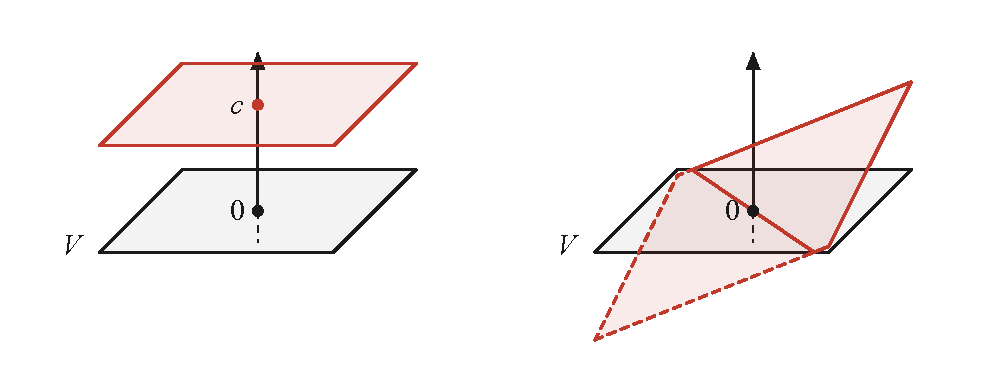
\includegraphics[width=0.84\textwidth]{figures/const-vs-linear.pdf}
\caption*{Рис. 2. Простейшие поверхности над плоскостью $V$. Слева — константа: горизонтальная плоскость на высоте $c$. Справа — линейная функция: наклонная плоскость, проходящая через $0$; красная прямая — то место, где она пересекает $V$ (часть плоскости под $V$ показана штрихами).}
\end{figure}

\section{Линейные формы}

\subsection{Определение}

Функция $f\colon V \to \mathbb{R}$ называется \textbf{линейной}, если
\[
\begin{aligned}
&f(\vec a + \vec b) = f(\vec a) + f(\vec b) &&\forall\, \vec a, \vec b \in V, \\
&f(\lambda \vec a) = \lambda f(\vec a) &&\forall\, \vec a \in V,\ \forall\, \lambda \in \mathbb{R}.
\end{aligned}
\]

Это стандартные условия, которые всегда называют линейностью. Как обычно, знаки операций в разных частях равенств имеют разную природу: в левой части первого равенства складываются векторы, в правой — числа; в левой части второго вектор умножается на число внутри $V$, в правой перемножаются два числа. Оба условия можно объединить в одно, $f(\alpha \vec a + \beta \vec b) = \alpha f(\vec a) + \beta f(\vec b)$ для любых $\vec a, \vec b \in V$ и $\alpha, \beta \in \mathbb{R}$, но мы будем пользоваться записью в две строки: в ней явно видна линейность по каждой операции — по сложению и по умножению на число.

Из второго условия при $\lambda = 0$ сразу следует
\[
f(\vec 0) = 0,
\]
т. е. любая линейная функция обращается в нуль на нулевом векторе. Это необходимое условие линейности.

\subsection{График линейной функции — плоскость через ноль}

Вернёмся к геометрическим векторам на плоскости и убедимся, что абстрактно-алгебраическое определение приводит к картинке рис. 2.

Введём на плоскости какой-нибудь базис $\{\vec e_1, \vec e_2\}$. Можно взять ортонормированный — тогда координаты вектора будут обычными декартовыми координатами $x, y$, — но ортонормированность для рассуждения не нужна. Каждый вектор раскладывается по базису, $\vec a = \alpha_1 \vec e_1 + \alpha_2 \vec e_2$, и тем самым описывается столбцом $(\alpha_1, \alpha_2)$. Это снова изоморфизм: делать операции со столбцами — всё равно что делать их с самими векторами. Умножив на $2$ столбец $(2, 1)$, мы получим столбец $(4, 2)$, и он изображает ровно тот вектор, который получится, если умножить на $2$ вектор со столбцом $(2, 1)$; то же со сложением. Мы этого обычно не замечаем, но в этом и состоит изоморфизм.

Пусть $f$ линейна. Для любого вектора $\vec a$
\[
f(\vec a) = f(\alpha_1 \vec e_1 + \alpha_2 \vec e_2) = f(\alpha_1 \vec e_1) + f(\alpha_2 \vec e_2) = \alpha_1 \underbrace{f(\vec e_1)}_{A} + \alpha_2 \underbrace{f(\vec e_2)}_{B}.
\]

Первое равенство верно для любой функции: мы просто подставили разложение аргумента. Второе — следствие первого условия линейности, третье — второго. Числа $A = f(\vec e_1)$ и $B = f(\vec e_2)$ — какие-то фиксированные числа. Обозначив значение $z = f(\vec a)$, получаем
\[
A \alpha_1 + B \alpha_2 - z = 0.
\]

Это уравнение плоскости в координатах $(\alpha_1, \alpha_2, z)$. В аналитической геометрии плоскость задают уравнением $Ax + By + Cz + D = 0$; у нас $C = -1$, а $D = 0$, т. е. плоскость проходит через начало координат. Итак, график любой линейной функции — плоскость через ноль, а значения функции на базисных векторах играют роль коэффициентов в уравнении этой плоскости.

Верно и обратное. Пусть значения функции лежат на невертикальной плоскости, проходящей через ноль: $Ax + By + Cz = 0$, $C \neq 0$. Если вектору со столбцом $(x_1, y_1)$ соответствует значение $z_1$, а вектору $(x_2, y_2)$ — значение $z_2$, то
\[
A x_1 + B y_1 + C z_1 = 0, \qquad A x_2 + B y_2 + C z_2 = 0.
\]

Сложив эти равенства, получим $A(x_1 + x_2) + B(y_1 + y_2) + C(z_1 + z_2) = 0$: сумме векторов (её столбец — $(x_1 + x_2, y_1 + y_2)$) соответствует сумма значений. Это первое условие линейности. Умножив первое равенство на $\lambda$, получим второе: если взять вектор в пять раз длиннее, то и на плоскости нужно попасть в пять раз выше, туда мы и попадаем.

\subsection{Почему «форма»}

Линейные функции на линейном пространстве называют также \textbf{линейными формами}. Слово «отображение» применимо к совершенно любым множествам: можно отображать множество видов улиток, обитающих где-нибудь, в множество слов словаря, сопоставляя виду его название. Функцией обычно называют отображение из одного числового множества в другое ($\mathbb{R} \to \mathbb{R}$, $\mathbb{R} \to \mathbb{C}$, $\mathbb{C} \to \mathbb{R}$, …). Оператор переводит функцию в функцию, функционал — функцию в число. Слово «форма» используют, когда из вектора, т. е. из элемента линейного пространства, делают число. Ошибкой не будет сказать и «функция»; слово «форма» лишь подчёркивает природу аргумента. Сегодня «линейная форма» и «линейная функция» для нас синонимы.

Ещё раз о том, зачем мы этим занимаемся. Во-первых, это самое простое, что бывает из нетривиального. Во-вторых, это очень полезно. Наша исходная мысль была строить функции из $V$ в $V$, но если детально разбираться с ними, быстро оказывается, что без линейных форм $V \to \mathbb{R}$ не обойтись: можно делать вид, что их там нет, но при подробном разборе они возникают именно там. Поэтому и важно, чтобы мы отображали в то поле, над которым определено линейное пространство.

\section{Как изображают линейные формы: линии уровня}

Обычно линейные формы рисуют не так, как на рис. 2. Если речь идёт о геометрических векторах на плоскости, то и форму удобно изобразить на той же плоскости.

\subsection{Векторы, на которых форма равна нулю}

Мы уже знаем, что $f(\vec 0) = 0$. Утверждается, что найдётся и \emph{ненулевой} вектор $\vec v$, для которого $f(\vec v) = 0$.

Возьмём наугад какой-нибудь вектор $\vec a$. Если $f(\vec a) = 0$, нам просто повезло. Скорее всего, повезёт не сразу, и $f(\vec a) = \alpha \neq 0$. Тогда по второму условию линейности
\[
f\Big(\frac{\vec a}{\alpha}\Big) = \frac{1}{\alpha} f(\vec a) = 1.
\]

Возьмём теперь вектор $\vec b$, не коллинеарный $\vec a$ (для этого размерность должна быть не меньше двух). Если $f(\vec b) = 0$, мы снова закончили; если $f(\vec b) = \beta \neq 0$, то точно так же $f(\vec b/\beta) = 1$. Обозначим $\vec a^{\,\prime} = \vec a/\alpha$ и $\vec b^{\,\prime} = \vec b/\beta$; на обоих форма равна единице. Значит, на их разности она равна нулю:
\[
\vec v = \vec a^{\,\prime} - \vec b^{\,\prime} = \frac{\vec a}{\alpha} - \frac{\vec b}{\beta}, \qquad f(\vec v) = 1 - 1 = 0,
\]
причём $\vec v \neq \vec 0$, потому что $\vec a$ и $\vec b$ мы специально брали неколлинеарными.

Найдя один такой вектор, мы сразу получаем целую прямую: $f(2\vec v) = 0$ и вообще $f(\lambda \vec v) = \lambda f(\vec v) = 0$ для любого $\lambda$. Все векторы, концы которых лежат на этой прямой, форма переводит в нуль (рис. 3).

\subsection{Стопка линий уровня}

Точно так же можно найти все векторы, на которых форма равна единице. Один такой у нас есть — $\vec a^{\,\prime}$. Прибавим к нему $\vec v$:
\[
f(\vec a^{\,\prime} + \vec v) = f(\vec a^{\,\prime}) + f(\vec v) = 1 + 0 = 1,
\]
и вообще $f(\vec a^{\,\prime} + \lambda \vec v) = 1$ при любом $\lambda$. Получается прямая, параллельная нулевой, только немного отставленная от неё. Аналогично векторы $-\vec a^{\,\prime} + \lambda \vec v$ дают прямую, на которой форма равна $-1$, векторы $2\vec a^{\,\prime} + \lambda \vec v$ — прямую со значением $2$, и т. д. Все эти прямые параллельны и расположены на равных расстояниях друг от друга. Получается то, что называют \textbf{стопкой} линий уровня (рис. 3).

\begin{figure}[H]
\centering
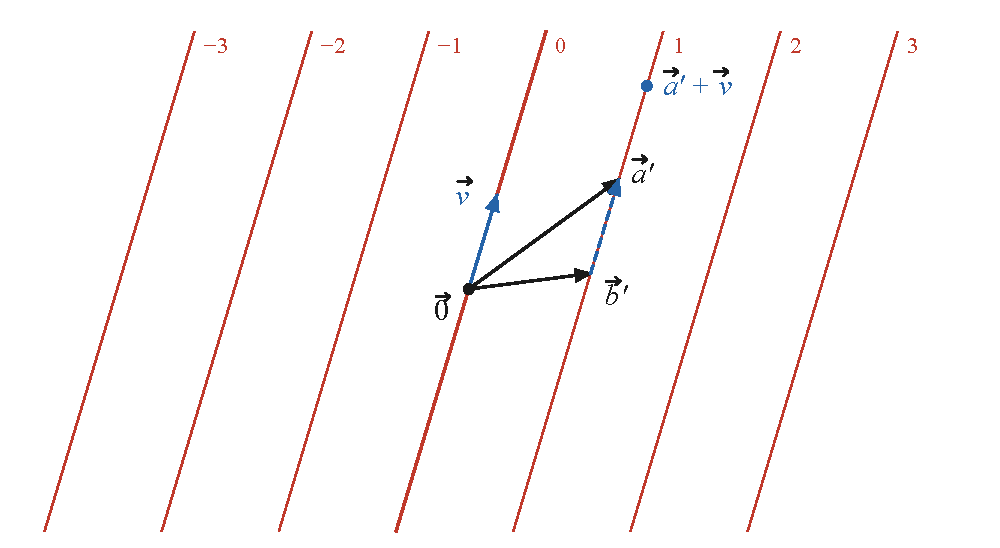
\includegraphics[width=0.84\textwidth]{figures/level-lines.pdf}
\caption*{Рис. 3. Линейная форма на плоскости — стопка параллельных равноотстоящих прямых; числа — значения формы на них. Векторы $\vec a^{\,\prime}$ и $\vec b^{\,\prime}$ оканчиваются на прямой $f = 1$, поэтому их разность $\vec v$ (синяя) лежит на прямой $f = 0$; прибавляя $\vec v$ к $\vec a^{\,\prime}$, мы остаёмся на прямой $f = 1$.}
\end{figure}

Важно понимать, что вся эта картинка нарисована в самом линейном пространстве — не снаружи и не где-то ещё. Красная прямая «закрашивает» концы всех векторов, которые данная функция $f$ переводит в нуль; соседняя — концы всех векторов, которые она переводит в единицу.

\subsection{Связь с графиком}

Как эта картинка соотносится с прежней, трёхмерной? Там мы откладывали значения формы по третьей оси и получали наклонную плоскость через ноль. Проведём на этой плоскости горизонтальные сечения на высотах $1, 2, -1, \dots$ и спроецируем их на $V$. Получатся ровно наши равноотстоящие прямые (рис. 4): стопка — это проекции линий уровня графика на само линейное пространство.

\begin{figure}[H]
\centering
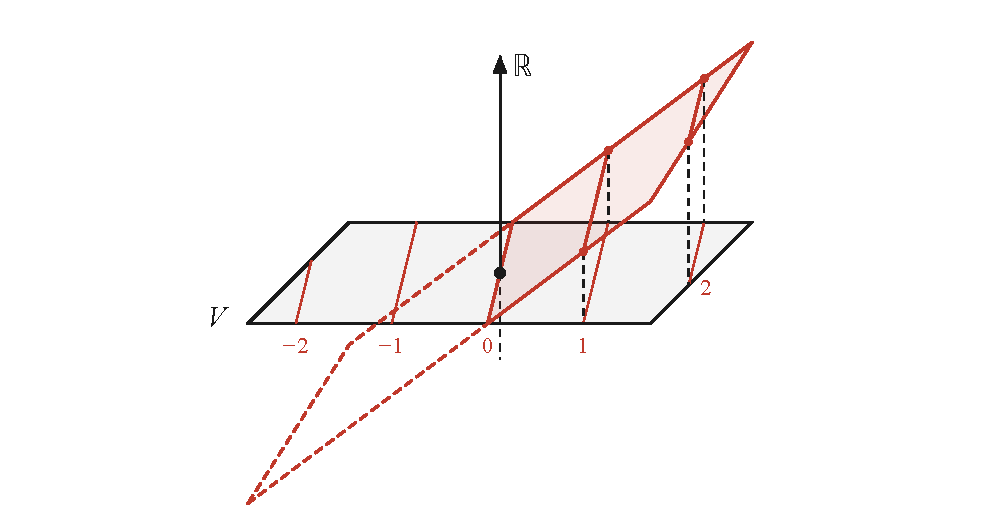
\includegraphics[width=0.84\textwidth]{figures/plane-sections.pdf}
\caption*{Рис. 4. График линейной функции и её линии уровня. Сечения наклонной плоскости на высотах $1$ и $2$ проектируются на $V$ в прямые $f = 1$ и $f = 2$; все прямые $f = c$ параллельны и идут с одинаковым шагом.}
\end{figure}

\subsection{Сколько информации хранит линейная форма}

Что такое вектор? Стрелочка. Но вектором вектор делает не стрелочка, а способность складываться с себе подобными: сила тока в цепи хоть и рисуется со стрелкой, вектором не является (об этом шла речь во второй лекции). Подумаем теперь о векторе с точки зрения содержащейся в нём информации. В двумерном векторе информации ровно на два действительных числа, в $n$-мерном — на $n$ чисел. Как учат физики, у вектора есть длина и направление: на плоскости направление задаётся одним углом, в пространстве — двумя, так что в сумме получается два и три числа соответственно.

Чем могут отличаться друг от друга две линейные формы на плоскости? Обе стопки обязательно проходят через ноль. Отличаться они могут, во-первых, ориентацией — она тоже задаётся одним числом, — а во-вторых, расстоянием между линиями уровня (рис. 5). Итого два числа. В трёхмерном пространстве понадобилось бы три: одно на расстояние и два на ориентацию. Получается, что в линейной форме хранится столько же информации, сколько в векторе.

\begin{figure}[H]
\centering
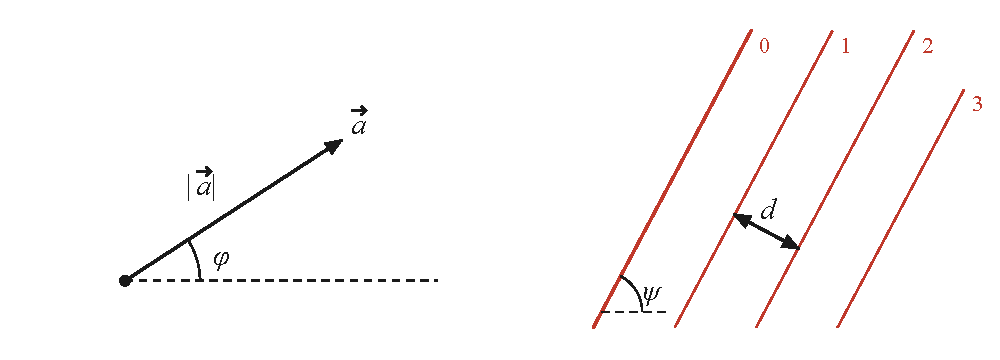
\includegraphics[width=0.84\textwidth]{figures/information.pdf}
\caption*{Рис. 5. Слева — вектор: длина $|\vec a|$ и направление (угол $\varphi$). Справа — линейная форма: шаг $d$ между линиями уровня и их наклон (угол $\psi$). И там, и там по два числа.}
\end{figure}

Рассуждение про расстояния и углы годится, конечно, только для геометрических векторов; в абстрактном пространстве непонятно, что такое расстояние между линиями уровня. Алгебраическая формулировка — обобщение многих реализаций одного факта в разных пространствах, и до неё надо дорасти, поэтому мы сначала щупаем факт в привычной геометрии. Но сам факт верен для любых линейных форм на любом конечномерном пространстве. Например, на пространстве многочленов (скажем, степени не выше заданной) линейную форму задаёт интеграл: многочлену $p$ сопоставляется число $\int_a^b p(x)\,dx$. Интегрирование — линейная операция, оба условия определения выполнены. Стопкой такую форму вряд ли нарисуешь, но формально она подходит под определение, и в ней, как мы увидим, тоже хранится ровно столько информации, сколько в многочлене.

% ПРОВЕРИТЬ 00:45:52: в записи «считаю интеграл от АДБ, получаю число», восстановлено как интеграл от a до b

Если эти соображения ни на какие мысли не навели, их можно просто забыть. Если навели — давайте их формализуем.

\section{Сопряжённое пространство}

Мера информации в векторе — $n$ действительных чисел. Утверждается, что и линейная форма на $n$-мерном пространстве однозначно задаётся $n$ числами. Это возможно благодаря двум фактам.

\begin{enumerate}
\item Линейные формы на $V$ образуют линейное пространство в абстрактном смысле — в смысле определения, данного на второй лекции. Оно обозначается $V^*$ и называется \textbf{сопряжённым} пространством (говорят также двойственное, дуальное, иногда взаимное; мы обычно будем говорить «сопряжённое»).
\item Размерность сопряжённого пространства совпадает с размерностью исходного:
\end{enumerate}

\[
\dim V^* = \dim V.
\]

Это равенство и выражает ту идею, что в векторе и в линейной форме информация хранится одинаково.

\subsection{$V^*$ — линейное пространство}

Говорить, что множество «образует линейное пространство», не совсем правильно: оно образует линейное пространство относительно каких-то введённых на нём операций. Пока у нас есть только множество линейных функций, и операции сложения и умножения на число на нём надо сначала определить, а затем проверить аксиомы. Конечномерность пространства $V$ здесь, кстати, не нужна.

Пусть $f, g \in V^*$ (мы немного забегаем вперёд: пока $V^*$ — просто множество всех линейных функций на $V$). Функцию $h = f + g$, $h\colon V \to \mathbb{R}$, определим так:
\[
h(\vec a) = f(\vec a) + g(\vec a) \qquad \forall\, \vec a \in V,
\]
а функцию $h = \lambda f$, где $\lambda \in \mathbb{R}$, — так:
\[
h(\vec a) = \lambda f(\vec a) \qquad \forall\, \vec a \in V.
\]

Чтобы объяснить, как устроена функция, нужно сказать, как она действует на любой аргумент, — именно это мы и сделали. Никакой магии: это единственные определения сложения функций и умножения функции на число, которые вообще приходят на ум.

Аксиомы линейного пространства для таких операций проверяются на значениях функций, где они сводятся к свойствам действительных чисел. Содержательная часть проверки — убедиться, что операции не выводят из множества линейных функций. Докажем, что сумма $h = f + g$ линейных функций линейна. Пользуемся определением суммы, затем линейностью $f$ и $g$, затем снова определением суммы:
\[
\begin{aligned}
h(\vec a + \vec b) &= f(\vec a + \vec b) + g(\vec a + \vec b) = f(\vec a) + f(\vec b) + g(\vec a) + g(\vec b) = h(\vec a) + h(\vec b), \\
h(\alpha \vec a) &= f(\alpha \vec a) + g(\alpha \vec a) = \alpha f(\vec a) + \alpha g(\vec a) = \alpha\, h(\vec a).
\end{aligned}
\]

То, что произведение линейной функции на число линейно, доказывается так же, только ещё проще. Проделайте это руками сами: смотреть, как это делает кто-то другой, пользы не приносит.

Итак, $V^*$ — линейное пространство. Заметим, зачем мы так долго обсуждали абстрактные линейные пространства. Тензоры тоже окажутся функциями, линейными в некотором смысле, — полилинейными, т. е. линейными по каждому аргументу, — и про них тоже можно будет доказать, что они образуют линейное пространство. А значит, на них автоматически переносится всё, что мы знаем о произвольных линейных пространствах, и в первую очередь существование базиса.

Второй факт, $\dim V^* = \dim V$, мы докажем, построив в $V^*$ специальный базис. Это частый приём: выбирается какой-то базис, с его помощью доказывается факт, а потом проверяется, что от выбора базиса ничего не зависело.

\section{Взаимный базис}

\subsection{Обозначения}

Элементы пространства $V$ мы обозначаем буквами со стрелкой: $\vec a$, $\vec b$, базис — $\vec e_1, \vec e_2, \dots$ Стрелка ставится у любых векторов, независимо от природы пространства: если $V$ — пространство многочленов, то запись $\vec p = x^2 + 1$ вполне законна. В книгах векторы печатают жирным шрифтом и спутать число с вектором там невозможно, а на письме возможно; стрелка нужна, чтобы путаницы точно не было.

Для элементов сопряжённого пространства разные источники используют разные обозначения; эта тема вообще гораздо меньше освещена в литературе. Мы будем обозначать их буквами (обычно греческими) с тильдой: $\tilde\omega$, $\tilde f$. У векторов — стрелка, у линейных форм — тильда.

\subsection{Идея: компоненты формы — её значения на базисе}

Сколько элементов в базисе $V^*$? Соображение про информацию доказательством, конечно, не является. В этом курсе мы почти везде не просто изучаем факты, но и обсуждаем, как к ним можно было бы прийти самостоятельно: как и с определителем в прошлой лекции, интересно не только \emph{что}, но и \emph{откуда берётся}.

Как абстрактное линейное пространство, $V^*$ имеет бесконечно много базисов, и ни один не лучше другого. (В геометрическом пространстве дополнительная структура — углы и длины — выделяет ортонормированные базисы, в каком-то смысле лучшие, чем остальные; в чистом линейном пространстве все базисы равноправны.) Но $V^*$ — не просто абстрактное пространство: оно построено на основе $V$ и как-то с ним связано. Этим и воспользуемся: если в $V$ уже выбран базис, то в $V^*$ можно выбрать вполне определённый, в каком-то смысле хороший базис. Попутно мы докажем, что в нём ровно $n$ элементов.

Чтобы не писать лишнего, возьмём $n = 3$; общий случай ничем не отличается. Пусть в $V$ зафиксирован базис $\{\vec e_1, \vec e_2, \vec e_3\}$, и пусть $\tilde f \in V^*$ — произвольная линейная форма. Она берёт вектор $\vec a = \alpha_1 \vec e_1 + \alpha_2 \vec e_2 + \alpha_3 \vec e_3$ и выдаёт число; по линейности можно раскрыть все скобки:
\[
\tilde f(\vec a) = \tilde f(\alpha_1 \vec e_1 + \alpha_2 \vec e_2 + \alpha_3 \vec e_3) = \alpha_1 \tilde f(\vec e_1) + \alpha_2 \tilde f(\vec e_2) + \alpha_3 \tilde f(\vec e_3).
\]

Обозначим
\[
\gamma_1 = \tilde f(\vec e_1), \qquad \gamma_2 = \tilde f(\vec e_2), \qquad \gamma_3 = \tilde f(\vec e_3).
\]

Видно, что информации здесь ровно на три действительных числа: функция $\tilde f$ целиком задаётся своим действием на базисные векторы. Зная три числа $\gamma_i$, можно объяснить другому человеку, как $\tilde f$ действует на любой вектор: разложи вектор по базису и подставь в формулу. Обратно, любые три числа $\gamma_1, \gamma_2, \gamma_3$ задают по этой формуле линейную форму. Таким образом, выбор базиса в $V$ порождает изоморфизм пространства линейных форм с тройками чисел.

Идея взаимного базиса рождается, когда, глядя на эту формулу, спрашиваешь: нельзя ли интерпретировать числа $\gamma_i$ как \emph{компоненты} формы $\tilde f$ в некотором базисе пространства $V^*$? Построим такие формы $\tilde\omega_1, \tilde\omega_2, \tilde\omega_3$, чтобы
\[
\tilde f = \gamma_1 \tilde\omega_1 + \gamma_2 \tilde\omega_2 + \gamma_3 \tilde\omega_3.
\]

Подчеркнём: раскладывается не значение $\tilde f$, а сама функция $\tilde f$ — как элемент линейного пространства $V^*$. Базис в этом пространстве состоит из функций, а сложение функций и умножение их на число мы определили как раз для того, чтобы любую функцию можно было представить в виде линейной комбинации других функций. Понятно, что такие $\tilde\omega_i$ будут зависеть от выбора базиса $\vec e_1, \vec e_2, \vec e_3$.

\subsection{Определение взаимного базиса}

Строим первую форму так, чтобы на первом базисном векторе она давала единицу, а на остальных — нуль; вторую — чтобы единицу она давала на втором; и т. д.:
\[
\begin{aligned}
&\tilde\omega_1(\vec e_1) = 1, \qquad \tilde\omega_1(\vec e_2) = \tilde\omega_1(\vec e_3) = 0, \\
&\tilde\omega_2(\vec e_2) = 1, \qquad \tilde\omega_2(\vec e_1) = \tilde\omega_2(\vec e_3) = 0, \\
&\tilde\omega_3(\vec e_3) = 1, \qquad \tilde\omega_3(\vec e_1) = \tilde\omega_3(\vec e_2) = 0.
\end{aligned}
\]

Для произвольного $n$ строк было бы $n$. Коротко всё это записывается с помощью символа Кронекера:
\[
\tilde\omega_i(\vec e_j) = \delta_{ij}. \tag{1}
\]

Набор линейных форм $\tilde\omega_1, \dots, \tilde\omega_n$, удовлетворяющих (1), называется \textbf{взаимным базисом} к базису $\vec e_1, \dots, \vec e_n$ (говорят также «двойственный базис»). Это определение по построению, а не что-то свалившееся с небес.

Однозначно ли это задаёт функции? Да. Мы только что видели, что при выбранном базисе в $V$ линейная форма задаётся своими значениями на $\vec e_1, \vec e_2, \vec e_3$, а эти значения могут быть любыми тремя числами. Значит, $\tilde\omega_1$ — та единственная линейная форма, значения которой на $\vec e_1, \vec e_2, \vec e_3$ равны $1, 0, 0$: такая форма в $V^*$ существует и единственна, мы её и берём. В частности, линейность $\tilde\omega_1$ отдельно доказывать не нужно: мы с самого начала выбираем её среди элементов $V^*$, т. е. среди линейных функций. Как она действует на произвольный вектор, видно по линейности:
\[
\tilde\omega_1(\vec a) = \tilde\omega_1(\alpha_1 \vec e_1 + \alpha_2 \vec e_2 + \alpha_3 \vec e_3) = \alpha_1 \cdot 1 + \alpha_2 \cdot 0 + \alpha_3 \cdot 0 = \alpha_1,
\]
и вообще $\tilde\omega_i(\vec a) = \alpha_i$: $i$-я форма взаимного базиса выдаёт $i$-ю компоненту вектора (рис. 6).

\begin{figure}[H]
\centering
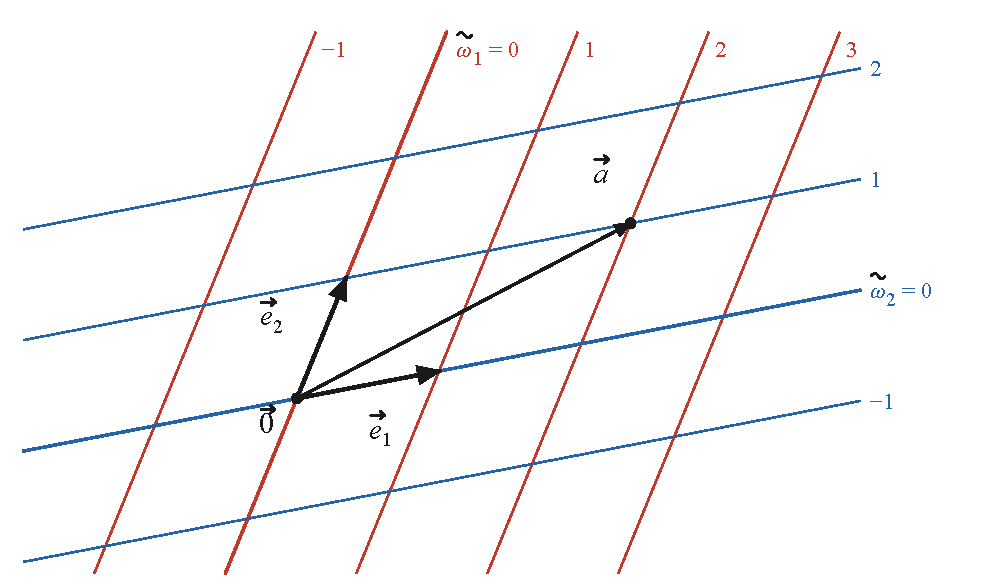
\includegraphics[width=0.84\textwidth]{figures/dual-basis.pdf}
\caption*{Рис. 6. Взаимный базис на плоскости. Линии уровня $\tilde\omega_1$ (красные) параллельны $\vec e_2$ и проходят через концы векторов $\vec 0, \vec e_1, 2\vec e_1, \dots$; линии уровня $\tilde\omega_2$ (синие) параллельны $\vec e_1$. Поэтому $\tilde\omega_1(\vec e_1) = 1$, $\tilde\omega_1(\vec e_2) = 0$ и т. д., а для $\vec a = 2\vec e_1 + \vec e_2$ формы выдают его компоненты: $\tilde\omega_1(\vec a) = 2$, $\tilde\omega_2(\vec a) = 1$.}
\end{figure}

\subsection{Разложение формы по взаимному базису}

Проверим, что цель достигнута. Объединяя разложение $\tilde f = \gamma_1 \tilde\omega_1 + \gamma_2 \tilde\omega_2 + \gamma_3 \tilde\omega_3$ с тем, что $\gamma_i = \tilde f(\vec e_i)$, мы хотим доказать, что
\[
\tilde f = \tilde f(\vec e_1)\, \tilde\omega_1 + \tilde f(\vec e_2)\, \tilde\omega_2 + \tilde f(\vec e_3)\, \tilde\omega_3. \tag{2}
\]

Здесь $\tilde f(\vec e_1)$ — не произведение, а результат действия $\tilde f$ на $\vec e_1$, т. е. число; $\tilde\omega_1$ — функция. Справа стоит линейная комбинация функций с числовыми коэффициентами.

На слово верить не надо, проверим. Равенство (2) — это равенство функций, а функции равны, если на любом аргументе они принимают одинаковые значения. Возьмём любой $\vec a \in V$. Левая часть, как мы уже выяснили, даёт
\[
\tilde f(\vec a) = \alpha_1 \tilde f(\vec e_1) + \alpha_2 \tilde f(\vec e_2) + \alpha_3 \tilde f(\vec e_3).
\]

Правая часть на векторе $\vec a$ даёт
\[
\tilde f(\vec e_1)\, \tilde\omega_1(\vec a) + \tilde f(\vec e_2)\, \tilde\omega_2(\vec a) + \tilde f(\vec e_3)\, \tilde\omega_3(\vec a) = \tilde f(\vec e_1)\, \alpha_1 + \tilde f(\vec e_2)\, \alpha_2 + \tilde f(\vec e_3)\, \alpha_3,
\]
поскольку $\tilde\omega_i(\vec a) = \alpha_i$. Получилось одно и то же, равенство (2) доказано. Мы пользовались линейностью форм $\tilde\omega_i$ — законно, ведь это элементы $V^*$, т. е. линейные функции.

Итак, во взаимном базисе компоненты линейной формы находятся очень просто: это её значения на базисных векторах, $\gamma_i = \tilde f(\vec e_i)$.

\subsection{Размерность сопряжённого пространства}

Мы доказали, что любая линейная форма раскладывается по $\tilde\omega_1, \dots, \tilde\omega_n$:
\[
\tilde f = \gamma_1 \tilde\omega_1 + \gamma_2 \tilde\omega_2 + \dots + \gamma_n \tilde\omega_n.
\]

Чтобы этот набор был базисом, осталось доказать его линейную независимость. Это совсем легко и оставляется читателю. Напомним, что линейную независимость можно определять через разложение нуля в линейную комбинацию — тривиальную или нетривиальную. Нуль здесь — это нуль того пространства, в котором всё происходит, т. е. $V^*$; обозначим его $\tilde 0$. Это тоже какая-то функция. Подумайте, почему нулём пространства $V^*$ является функция, выдающая $0$ на любом векторе (для этого надо вспомнить, что в аксиомах называется нулём). Дальше, как обычно, приравниваем линейную комбинацию форм $\tilde\omega_i$ к $\tilde 0$.

В итоге $\tilde\omega_1, \dots, \tilde\omega_n$ — базис пространства $V^*$, взаимный к базису $\vec e_1, \dots, \vec e_n$ пространства $V$. В нём $n$ элементов, следовательно,
\[
\dim V^* = n = \dim V.
\]

Взаимный базис — не единственный возможный базис в $V^*$, но общепринято брать именно его. Так будет и с тензорами: их можно построить целиком из прямого и сопряжённого пространства (возможно, вы уже видели запись вроде тензорного произведения $V^* \otimes V$), и чтобы говорить о компонентах тензора, в каждом пространстве нужен базис. В сопряжённом пространстве при этом молча берётся взаимный базис. Можно взять и другой, и для каких-то задач это, может быть, удобно, но так не принято.

\section{Замена базиса и верхние и нижние индексы}

\subsection{Напоминание: замена базиса в $V$}

Чтобы полностью описать переход от базиса $\{\vec e_1, \dots, \vec e_n\}$ к новому базису $\{\vec e^{\,\prime}_1, \dots, \vec e^{\,\prime}_n\}$, нужно каждый новый базисный вектор разложить по старым. Получается $n^2$ чисел — матрица $A = (a_{ij})$; обратный переход описывается матрицей $B = (b_{ij})$, и эти матрицы взаимно обратны:
\[
\vec e^{\,\prime}_i = \sum_{j=1}^n \vec e_j\, a_{ji}, \qquad \vec e_i = \sum_{j=1}^n \vec e^{\,\prime}_j\, b_{ji}.
\]

Один и тот же вектор $\vec v$ раскладывается и по старому, и по новому базису:
\[
\vec v = \sum_{i=1}^n v_i\, \vec e_i = \sum_{j=1}^n v'_j\, \vec e^{\,\prime}_j,
\]
и чтобы это было правдой, компоненты должны быть связаны не как попало. В прошлой лекции мы получили
\[
v'_i = \sum_{j=1}^n b_{ij}\, v_j, \qquad v_i = \sum_{j=1}^n a_{ij}\, v'_j.
\]

Базисные векторы пересчитываются прямой матрицей, а компоненты вектора — обязательно обратной: если базисные векторы растянулись в три раза, то компоненты нужно сжать в три раза, чтобы их линейная комбинация дала тот же самый вектор $\vec v$.

Почему в одних формулах стоит $a_{ji}$, а в других $a_{ij}$? Вопрос не в выборе: есть функции и правила работы с ними, и по этим правилам формулы выводятся строго. Другое дело — как их запоминать. Базисные векторы удобно представлять строкой, а компоненты — столбцом; строку, чтобы получить строку, умножают на матрицу справа: $\vec e^{\,\prime} = \vec e A$. Мы же учимся писать всё в индексах, потому что для тензоров матричная запись будет уже невозможна.

\subsection{Как меняется взаимный базис}

При замене базиса в $V$ базис в $V^*$ можно и не трогать, ничего страшного не произойдёт. Но предположим, что мы решили отныне и впредь при каждой замене базиса в $V$ пересчитывать базис в $V^*$ так, чтобы он оставался взаимным. Возня с пересчётом стоит того: взаимный базис действительно удобен (мы уже видели, как просто в нём находятся компоненты формы). Итак, мы хотим, чтобы наряду с
\[
\tilde\omega_i(\vec e_j) = \delta_{ij}
\]
выполнялось
\[
\tilde\omega'_i(\vec e^{\,\prime}_j) = \delta_{ij}.
\]

Новые формы $\tilde\omega'_i$ — элементы $V^*$, поэтому раскладываются по старому базису с какими-то коэффициентами: как и любая замена базиса в линейном пространстве, этот переход описывается $n^2$ числами. Запишем
\[
\tilde\omega'_i = \sum_{k=1}^n c_{ik}\, \tilde\omega_k
\]
с пока неизвестной матрицей $C = (c_{ik})$. Подставим в условие взаимности это разложение и разложение $\vec e^{\,\prime}_j = \sum_{\ell} \vec e_\ell\, a_{\ell j}$. Индексы суммирования назовём $k$ и $\ell$, чтобы они не смешивались со свободными индексами $i$ и $j$:
\[
\begin{aligned}
\delta_{ij} = \tilde\omega'_i(\vec e^{\,\prime}_j)
&= \Big(\sum_{k=1}^n c_{ik}\, \tilde\omega_k\Big)\Big(\sum_{\ell=1}^n \vec e_\ell\, a_{\ell j}\Big)
= \sum_{k=1}^n c_{ik} \sum_{\ell=1}^n a_{\ell j}\, \tilde\omega_k(\vec e_\ell) \\
&= \sum_{k=1}^n c_{ik} \sum_{\ell=1}^n a_{\ell j}\, \delta_{k\ell}
= \sum_{k=1}^n c_{ik}\, a_{kj}.
\end{aligned}
\]

Обе суммы можно вынести. В первой лекции мы доказывали перестановочность сумм для чисел; здесь под знаком суммы стоят функции, но ничего незаконного нет: внешнюю сумму можно раскрыть по определению суммы функций, внутреннюю — по линейности каждой $\tilde\omega_k$. Если есть сомнения, распишите всё руками для $n = 2$ или $n = 3$. Далее, старый базис взаимный, поэтому $\tilde\omega_k(\vec e_\ell) = \delta_{k\ell}$, а сумма по $\ell$ с символом Кронекера $\delta_{k\ell}$ просто заменяет $\ell$ на $k$.

Получилось $\sum_k c_{ik}\, a_{kj} = \delta_{ij}$, т. е. в матричной записи $CA = E$. Значит, $C$ — матрица, обратная к $A$, т. е. $C = B$, $c_{ik} = b_{ik}$:
\[
\tilde\omega'_i = \sum_{j=1}^n b_{ij}\, \tilde\omega_j, \qquad \tilde\omega_i = \sum_{j=1}^n a_{ij}\, \tilde\omega'_j.
\]

Это главный результат: если базис $V$ пересчитывается прямой матрицей, то взаимный базис, чтобы оставаться взаимным, пересчитывается обратной. Это и интуитивно понятно: если, например, все базисные векторы растянуть втрое, то, чтобы по-прежнему $\tilde\omega'_i(\vec e^{\,\prime}_i) = 1$, формы придётся втрое уменьшить.

\subsection{Компоненты линейной формы}

Возьмём теперь отдельно взятую линейную форму $\tilde f$ и разложим её по старому и по новому взаимному базису: $\tilde f = \sum_i \gamma_i\, \tilde\omega_i = \sum_i \gamma'_i\, \tilde\omega'_i$. Вдумайтесь, какая это сложная конструкция: есть прямое пространство и сопряжённое к нему, в обоих есть базисы, причём взаимные; мы меняем базис в $V$, подстраиваем под него базис в $V^*$ так, чтобы он оставался взаимным, — и при этом как-то пересчитываются компоненты формы. Как именно — здесь всё наоборот по сравнению с компонентами вектора:
\[
\gamma'_i = \sum_{j=1}^n \gamma_j\, a_{ji}, \qquad \gamma_i = \sum_{j=1}^n \gamma'_j\, b_{ji}.
\]

Убедитесь самостоятельно, что эти формулы верны. Сложный вывод мы проделали вместе в п. 6.2, а остальное получается так же: сопряжённое пространство — такое же линейное пространство, и если базис в нём меняется матрицей $B$, то компоненты его элементов — обратной к ней матрицей $A$.

\subsection{Восемь формул}

Сведём всё вместе:

\begin{center}
\begin{tabular}{|c|c|c|}
\hline
 & Переход к новому базису & Обратный переход \\ \hline
Базисные векторы & $\vec e^{\,\prime}_i = \sum_{j=1}^n \vec e_j\, a_{ji}$ & $\vec e_i = \sum_{j=1}^n \vec e^{\,\prime}_j\, b_{ji}$ \\ \hline
Компоненты вектора & $v'_i = \sum_{j=1}^n b_{ij}\, v_j$ & $v_i = \sum_{j=1}^n a_{ij}\, v'_j$ \\ \hline
Взаимный базис & $\tilde\omega'_i = \sum_{j=1}^n b_{ij}\, \tilde\omega_j$ & $\tilde\omega_i = \sum_{j=1}^n a_{ij}\, \tilde\omega'_j$ \\ \hline
Компоненты формы & $\gamma'_i = \sum_{j=1}^n \gamma_j\, a_{ji}$ & $\gamma_i = \sum_{j=1}^n \gamma'_j\, b_{ji}$ \\ \hline
\end{tabular}
\end{center}

Обратные переходы (правый столбец) здесь не играют ключевой роли. Посмотрим на левый столбец. У нас четыре объекта: базисные векторы, компоненты отдельно взятого вектора в $V$, базисные формы и компоненты отдельно взятой формы в $V^*$. Два из них при переходе к новому базису пересчитываются прямой матрицей $A$ (базисные векторы и компоненты формы), два — обратной матрицей $B$ (компоненты вектора и взаимный базис). Величин стало вдвое больше, а новых матриц не появилось. Забегая вперёд, скажем, что и дальше ничего третьего не будет: когда появятся тензоры, мы по-прежнему будем иметь дело только с матрицами $A$ и $B$.

\subsection{Верхние и нижние индексы}

Отсюда и возникает идея: будем писать индексы снизу у всех величин, которые пересчитываются прямой матрицей, и сверху — у тех, которые пересчитываются обратной. Базисные векторы $\vec e_i$ и компоненты линейной формы $\gamma_i$ сохраняют нижние индексы, а компоненты вектора и формы взаимного базиса получают верхние: $v^i$, $\tilde\omega^i$.

Если вы раньше не встречали верхних и нижних индексов, пока может быть непонятно, зачем это нужно. Если встречали, но не понимали, откуда они берутся, — вот они, на ладони: так, по-видимому, рассуждали те, кто впервые начал их писать. Позже мы увидим, что у этой записи очень красивый смысл: с ней можно будет вообще опускать знаки сумм. С новой записью нужно сначала набить руку, поэтому в этой лекции формулы оставлены с нижними индексами; дальше мы продолжим эту тему.

\section{Ковекторы}

Элемент сопряжённого пространства называют также \textbf{ковектором}. Ковектор — просто синоним линейной формы; в зависимости от контекста эти слова могут иметь разный оттенок, но означают одно и то же.

Самый распространённый пример ковектора — градиент. О нём мы умышленно пока ничего не говорим. Градиент действительно является ковектором, но чтобы это понять, нужно проделать определённую работу: поговорить о многообразиях, функциях на них и т. д. Если просто сказать «градиент — ковектор, потому что он как-то там пересчитывается», понимание от этого только ухудшится. Поэтому разговор о градиенте отложим до тензорного анализа.

Чтобы пощупать, что такое ковектор, не обязательно говорить о градиенте: есть пример понятнее — плоская волна. Коэффициенты $\omega, k_x, k_y, k_z$, которые стоят в её выражении, — это компоненты некоторой линейной формы на четырёхмерном пространстве в некотором базисе. При пересадке в другую систему отсчёта, т. е. при замене базиса, они пересчитываются по формулам п. 6.4, и из этих формул можно получить, например, формулы эффекта Доплера для частоты и аберрации. Эту линию мы здесь развивать не будем, но она показывает, что вся эта линейная наука очень применима к жизни.

\emph{Замечание редактора.} Имеется в виду, что фаза плоской волны $\omega t - k_x x - k_y y - k_z z$ — линейная функция координат события $(t, x, y, z)$, т. е. линейная форма на четырёхмерном пространстве; с точностью до знаков её компоненты и есть $\omega, k_x, k_y, k_z$.

Следующая лекция тоже будет посвящена линейным формам, но уже на более абстрактном уровне.

\par\bigskip\noindent\rule{\textwidth}{0.4pt}\par\noindent \emph{Конец лекции 4.}

\end{document}
% checksum: a8c2731a4b522c833e379eaac2539b7666e23da0
